\chapter{Drasil}
\label{c:drasil}
%
%\ds{**Section Roadmap:
%    -- This is where the real meat of Drasil is discussed (implementation 
%details)
%    -- Intro to our knowledge-capture mechanisms
%      - Chunks/hierarchy
%      - Break down each with examples from the case studies.
%      - Look for 'interesting' examples (synonyms, acronyms, complexity, etc.)
%    -- Intro to the DSL
%      - Captured knowledge is useless without the transformations/rendering 
%engine
%      - DSL for each \sf{}}

In this chapter, we introduce the Drasil framework and its implementation 
details, including knowledge-capture mechanisms, the domain specific 
languages (DSLs) used throughout, and how these components are integrated 
in a human-usable way to generate \sfs{}. The name Drasil, derived from Norse 
Mythology's world tree Yggdrasil whose branches spread across the 
many realms, reflects how our framework spans the many domains and contexts 
relevant to software generation.
      
\section{Drasil in a nutshell}

Manually writing and maintaining a full range of \sfs{} is redundant, tedious, 
and often leads to divergent \sfs{}. Drasil is a purpose-built framework 
created to tackle these problems.

Unlike documentation generators like Doxygen, Javadoc, and Pandoc
which take a code-centric view of the problem and rely on manual redundancy -- 
i.e. natural-language explanations written as specially delimited
comments which can then be weaved into API documentation alongside code -- 
Drasil takes a knowledge-centric, redundancy-limiting, fully traceable, 
single-source approach to generating \sfs{}.

However, Drasil is not, nor is it intended to be, a panacea for all the woes of 
software development. Even the seemingly well-defined problems of unnecessary 
redundancy and manual duplication turn out to be large, many-headed beasts 
which exist across a multitude of software domains; each with their own 
benefits, drawbacks, and challenges.

To reiterate: Drasil has not been designed as a silver-bullet. It is a 
specialized tool meant to be used in well-understood domains for software that 
will undergo frequent maintenance and/or changes. In deciding whether Drasil 
would be useful for developing software to tackle a given problem, we recommend 
identifying those projects that are long-lived (10+ years) with \sfs{} 
relevant to multiple stakeholders. For our purposes, as mentioned earlier, we 
have focused on SC software that follows the input $\rightarrow$ process 
$\rightarrow$ output pattern. SC software has the benefit of being relatively 
slow to change, so models used today may not be updated or invalidated for some 
time, if ever. Should that happen, the models will likely still be applicable 
given a set of assumptions or assuming certain acceptable margins for error.

With Drasil being built around this specific class of problems, we remain aware 
that there are likely many in-built assumptions in its current state that could 
affect its applicability to other domains. As such, we consider expanding 
Drasil's reach as an avenue for future work.

The Drasil framework relies on a knowledge-centric approach to software 
specification and development. We attempt to codify the foundational theory 
behind the problems we are attempting to solve and operationalize it through 
the use of generative technologies. By doing so, we can reuse common knowledge 
across projects and maintain a single source of truth in our knowledge database.

Given how important knowledge is to Drasil, one might think we are building 
ontologies or ontology generators. We must make it clear this is \emph{not} the 
case. We are not attempting to create a source for all knowledge and 
relationships inside a given field. We are merely using the information we have 
available to build up knowledge as needed to solve problems. Over time, this 
may take on the appearance of an ontology, but Drasil does not currently 
enforce any strict rules on how knowledge should be captured, outside of its 
type system and some best practice recommendations. We will explore knowledge 
capture in more depth in Section~\ref{sec:kc}.

\section{Our Ingredients: Organizing and Capturing Knowledge}
\label{sec:kc}

For Drasil to function as intended, we need a means of capturing and organizing 
the underlying knowledge of the software systems we are trying to build 
alongside common knowledge that would be relevant across our entire target 
domain of SC software. This knowledge capture method must also be robust enough 
to be operationalized by a multi-faceted generation framework.

Before we can design a knowledge capture mechanism, we must first define what 
exactly we believe we need to capture. It is nearly impossible to consider 
every case of knowledge that could be used in the domain of SC software, not to 
mention an extremely large undertaking to begin with ``all the things". As 
such we have decided to take an iterative, progressive refinement approach to 
our knowledge capture mechanisms. This should come as no surprise and follows 
from our general process for developing the Drasil framework.

\subsection{Capturing Knowledge via Chunks}
\label{sec:kcChunk}

We begin by borrowing and re-purposing the \emph{chunk} term from Literate 
Programming (LP) and use it to create a simplified, extensible, and ever 
expanding hierarchy  of chunks based on the requirements for capturing a single 
piece of knowledge. Our base chunk, \codeH{NamedChunk} is defined in 
Figure~\ref{fig:namedchunk} and can be thought of as any uniquely identifiable 
term. It is composed of a \codeH{UID}, or unique identifier, and a 
\codeH{NP}, or noun phrase, representing the term.

\fig{
\lstinputlisting[language=Haskell, firstline=33, lastline=43, 
firstnumber=33]{code/NamedIdea.hs}}{NamedChunk Definition}{fig:namedchunk}

A single node does not a hierarchy make, but with the root \codeH{NamedChunk} 
defined, we can begin to progressively extend it to cover any new chunk types 
we may need for our knowledge capture requirements. For example, if we want to 
capture a simple term with its definition, we need more than just a 
\codeH{NamedChunk}. We need to extend \codeH{NamedChunk} to include a 
definition, and we refer to this particular variant chunk as a 
\codeH{ConceptChunk}. For ease of creation, we define a number of semantic, 
so-called \emph{smart constructors} for each chunk type which allow us to more 
simply define our chunks and their intermediary datatypes (ie: \codeH{UID} and 
\codeH{NP} from the \codeH{NamedChunk} example). An example of such smart 
constructors being used to create simple instances of \codeH{ConceptChunk} can 
be seen in Figure~\ref{fig:conceptchunk}. Note there are smart constructors 
for each datatype when multiple variants exist and could be used in a given 
place. Looking at the \codeH{ConceptChunk} example, we can see two different 
smart constructors (\codeH{cnIES} and \codeH{cn'}) being used to create the 
\codeH{NP} instance. Both smart constructors create an instance of \codeH{NP}, 
but in this case the smart constructor used defines given properties (ie. 
pluralization rules of the noun phrase used as a term) for the instance to 
simplify construction.

\fig{
\lstinputlisting[language=Haskell, firstline=76, 
lastline=82, firstnumber=76]{code/Math.hs}}{Some example instances of 
\codeH{ConceptChunk} 
using the \codeH{dcc} smart constructor}{fig:conceptchunk}

These simple chunks are fine as a starting point, however, knowing the SC 
domain we can already foresee the need for a variety of other chunks. For 
brevity, we will only expand upon the chunks needed for the examples used in 
this paper. More information, including detailed definitions of all the types 
and current state of Drasil can be found in the wiki 
(\href{https://github.com/JacquesCarette/Drasil/wiki/}
{https://github.com/JacquesCarette/Drasil/wiki/}) or the Haddock documentation 
which can be generated from the Drasil source code or found online at 
\href{https://jacquescarette.github.io/Drasil/docs/full/}
{https://jacquescarette.github.io/Drasil/docs/full/}

\subsection{Chunk Combinatorics}
\label{sec:chunky}
\ds{Would we call our chunk hierarchy a DSL? Or would the DSL be more along the 
lines of Expr and Sentence which make up our chunks?}

Even with extremely simple chunks we have seen the need for multiple chunk 
types and a number of ways to construct instances of those types. The more we 
extend our chunk hierarchy, the larger the number of possible combinations we 
will need to account for. This is not only relevant to chunks themselves, but 
also to the information they encode. Take, for instance, a term definition that 
relies on other terminology that has been captured. In our effort to reduce 
duplication and maintain a single source of information, we intend to be able 
to create chunks with references to other chunks such that the definition can 
use the known terminology.

To define a term with references to other terms, we need to ensure we are 
creating our definitions by projecting relevant knowledge into the definition, 
but also ensuring we have the flexibility to extend that knowledge. With that 
in mind, we created a Domain Specific Language (DSL) for creating and combining 
(English language) sentences aptly called \codeH{Sentence}. In its most basic 
form, \codeH{Sentence} will simply wrap a string. However, by defining a number 
of helper functions and other useful utilities, our \codeH{Sentence} DSL can be 
used to combine, change case, pluralize, and more. A simple example of a series 
of chunks that utilize the \codeH{Sentence} DSL to derive their definitions can 
be seen in Figure~\ref{fig:acceleration}. We use the \codeH{phrase} helper 
function to pull the appropriate sentence out of the \codeH{velocity} chunk and 
the combinator (\codeH{+:+}) to concatenate the sentences. Note that 
\codeH{position} uses a different smart constructor (for non-derived 
definitions) and so doesn't require the sentence constructor (\codeH{S}) around 
its definition.

\ds{\sout{Should I work in something about how we use lenses in here, as all 
complex chunks are instances of the simpler chunks they've been built from? Or 
is that getting too into the Haskell-specific details?} I've written something 
below}

We also make opportunistic use of composable accessors (commonly known in the 
Haskell ecosystem as ``lenses") to help manage complexity when combining and 
projecting chunks. Conceptually, these are lightweight, composable getters and 
setters that let us focus on the logical structure of a chunk (its name, 
symbol, sentence, expression, units, etc.) without repeatedly writing 
boilerplate navigation code for nested fields\footnote{Concrete lens usage and 
examples are available in the code found in the project repository for 
readers who want the implementation details.}. In practice they let us build 
derived chunks by projecting the subparts we need, update specific components 
(for instance a symbol or an attached unit) in a principled, immutable way, and 
compose transformations cleanly when constructing larger chunks from smaller 
ones. 

\fig{
\lstinputlisting[language=Haskell, linerange={59-60,135-136,174-175}, 
numbers=none]{code/Physics.hs}
}{Projecting knowledge into a chunk's definition}{fig:acceleration}

Looking back at our examples of the types of knowledge we are interested in 
from Figure~\ref{fig:gbrddq} we can see that the simple chunks we've defined so 
far do not even start to cover the full spectrum of our needs. We can see a lot 
of information missing such as a symbolic representation ($\hat{q}$) and 
equation ($\hat{q} = \frac{q(ab)^2}{Eh^4\text{GTF}}$). As that is a relatively
complex example, we will start by looking at something far simpler: Newton's 
2nd Law of motion\citep{Newton1687} which, roughly translated, states ``the net 
force on a body at any instant of time is equal to the body's acceleration 
multiplied by its mass or, equivalently, the rate at which the body's momentum 
is changing with time"  or as most physics students recognize it $F=ma$ 
provided we have definitions for $F$, $m$, and $a$.

To understand what exactly is missing, let us look at how we achieve an 
operational definition of \emph{Force} as a chunk in Drasil. To start, we can 
see we need a symbolic representation ($F$) and some way to define an equation. 
Also, each of force, mass, and acceleration are measured in some form of units 
($N$, $kg$, and $m/s^2$ respectively) which we will likely care to capture and 
keep track of. 

\fig{
\lstinputlisting[language=Haskell, linerange={91-92}, 
firstnumber=91]{code/Physics.hs}
}{The force \codeH{ConceptChunk}}{fig:forceCC}

\fig{
\lstinputlisting[language=Haskell, linerange={47-47,57-57}, 
numbers=none]{code/PhysicsQuantities.hs}
}{The force and acceleration \codeH{UnitalChunk}s}{fig:forceUC}

We start by building a \codeH{ConceptChunk} for the Force concept as seen in 
Figure~\ref{fig:forceCC}. It is built from a common noun (``force") and a 
definition. Next we need to capture the units of measurement to the force 
concept by defining what we have named a \codeH{UnitalChunk}. This definition 
for force can be seen in Figure~\ref{fig:forceUC}. Note that we are not 
re-defining force in this instance. We are instead using a smart constructor to 
build atop the existing force chunk (\codeH{CP.force}) and adding a symbolic 
representation (\codeH{vec cF}, which is shorthand for the selected vector 
representation\footnote{More on this in Section~\ref{sec:recipes}} of the 
capital letter \emph{F}). We also must capture the units used to measure force
(\codeH{newton}) which are defined in \codeH{Data.Drasil.SI_Units} and can be 
seen in Figure~\ref{fig:Data.Drasil.SI}. The SI Units are captured using 
another type of chunk known as a \codeH{UnitDefn} which are built atop a 
\codeH{ConceptChunk} and \codeH{UnitSymbol}. The \codeH{UnitSymbol} is also a 
chunk that can be one of several other chunk types.\footnote{For brevity we are 
glossing over many chunk definitions and the differences between them as there 
are a large variety in use for even simple examples. They are covered in more 
depth in the full technical documentation found on our github repository.}. 
Returning to the force \codeH{UnitalChunk}, the smart constructor \codeH{uc} we 
are using will assume we are working in the real number space. There are 
other smart constructors for other spaces, which are also captured using other 
chunks elsewhere in Drasil (see: \codeH{Language.Drasil.Space}).

\fig{
\lstinputlisting[language=Haskell, linerange={21-30}, 
firstnumber=21]{code/SI_Units.hs}
}{The fundamental SI Units as Captured in Drasil}{fig:Data.Drasil.SI}

\fig{
\lstinputlisting[language=Haskell, linerange={11-20}, 
firstnumber=11]{code/PhysicsUnits.hs}
}{Examples of chunks for units derived from other SI Unit chunks}{fig:accelU}

Now we approach the terms mass and acceleration in a similar manner. We capture 
each as a \codeH{ConceptChunk} (see Figure~\ref{fig:acceleration} for a 
reminder of how we captured acceleration's definition relative to velocity and 
thus relative to position). Then construct a \codeH{UnitalChunk} for each. 
Acceleration can be seen in Figure~\ref{fig:forceUC} and mass has a similar 
\codeH{UnitalChunk} that uses the \codeH{metre UnitDefn} chunk. More 
interestingly, the units for acceleration are derived from other units, and can 
be seen in Figure~\ref{fig:accelU} with some additional derived unit types 
(taken from \codeH{Data.Drasil.Units.Physics}).

Now we have almost everything we need to finish our definition of Newton's 
second law. Everything thus far has been defined in natural language using our 
\codeH{Sentence} DSL, but it is not well-suited to the one piece we are 
currently missing: a way to define expressions relating chunks in a universal 
\ds{language agnostic?} (mathematics) context \ds{/representation}.

\subsection{Relating Chunks via Expressions}
\label{sec:expr}

Continuing our Newton's Second Law example from Section~\ref{sec:chunky}, we 
need a means to capture how force is calculated. We know it is calculated 
relative to mass and acceleration, so we need a way to encode that, preferably 
in an operational manner. We also know acceleration is itself derived from 
time and velocity, which is derived from time and position.

When thinking about the types of information we would like to encode with 
expressions, we have some obvious candidates. We should be able to encode 
common arithmetic operations (addition, subtraction, multiplication, division, 
exponentiation, etc.), boolean operations (and, or, not, etc.), comparisons 
(equal, not equal, less than, greater than), trigonometric functions (sin, tan, 
cos, arctan, etc.), calculus (derivation, integration, etc.), and vector/matrix 
operations (dot product, cross product, etc.). For the sake of our example 
we'll focus on only those we need to define Newton's Second Law of motion: 
multiplication and derivatives.

\fig{
\lstinputlisting[language=Haskell, linerange={194-202}, 
firstnumber=194]{code/Expr.hs}
}{Defining real number multiplication in \codeH{Expr}}{fig:mulRe}

As an aside, we will elide details on how we arrived at the current 
implementation of the expression DSL known as \codeH{Expr}, but suffice to say 
it was driven by a practical, ``lowest common denominator" approach to 
developing the operations that could be encoded and factoring out commonalities 
much the same way we did with the rest of the case studies. With that in mind, 
we have encoded multiplication (for real numbers) as seen in 
Figure~\ref{fig:mulRe}. \codeH{AssocA} refers to an associative arithmetic 
operator which can be applied across a list of expressions (in this case, 
\codeH{mulRe}, though addition and other associative operations look very 
similar). Derivation is much simpler to encode, as it is simply a relationship 
between two existing chunks, ie. \codeH{deriv a b} represents taking the 
derivative of \codeH{a} with respect to \codeH{b}.

\fig{
\lstinputlisting[language=Haskell, linerange={16-16, 20-23}, 
numbers=none]{code/PhysicsEquations.hs}
}{Encoding Newton's second law of motion}{fig:newton}

Continuing our example, we see (Figure~\ref{fig:newton}) it is fairly trivial 
to encode the expression for Newton's Second Law using the \codeH{Expr} DSL. We 
are still not done building our Newton's Second Law chunk however, as this 
specific law should be referable by its own identifier. It is not simply 
``force", nor the relationship between mass and acceleration, but a combination 
of both with its own natural language semantics that allow us to refer to it 
specifically. The full definition for this particular chunk can then be found 
in Figure~\ref{fig:newtonChunk}. The chunk is defined relative to force and the 
expression captured in Figure~\ref{fig:newton}, alongside a new identifier and 
description. Notice we are building off of other chunks throughout each piece 
of the chunk's definition, thus giving us perfect traceability from beginning 
to end, regardless of whether we are looking at a defining expression or 
natural language description.

\fig{
\lstinputlisting[language=Haskell, linerange={34-42}, 
numbers=none]{code/PhysicsEquations.hs}
}{Newton's second law of motion as a \emph{Chunk}}{fig:newtonChunk}

The \codeH{Expr} DSL grants us flexibility in defining relationships without 
imposing any particular structure on a chunk other than ``contains an 
\codeH{Expr}", or more specifically ``can be modeled using an \codeH{Expr}." 
Our example also shows us that a few simple chunk types can be combined 
repeatedly to build much more robust, complex, and information-dense chunks. On 
the other hand, encoding even a relatively simple theory like Newton's Second 
Law of motion requires us to define chunks down to the fundamentals. 
Luckily, that is another area where chunks shine as they are infinitely 
reusable. Once a chunk has been defined and added to our knowledge-base, we 
never need to redefine it. We simply use it wherever it is needed.

On the topic of using chunks, we now need a means for taking our chunks and 
structuring them such that we can actually do something useful with them. For 
example, how would we go from chunks to \sfs{}? Look forward to that in 
Section~\ref{sec:recipes}.

\subsection{Chunk Classification}
%\ds{Prev title: ``Chunk Summary" and comment: I kind 
%of want to skip this section, though I can
%also understand keeping it. It does feel a little too ``in the weeds" to go 
%through the whole Chunk Hierarchy, but I do think it's worthwhile to include
%the kinds of things we can capture. Maybe a brief ``We've touched on Blah, and 
%we've also determined we need to be able to capture `blerb, flerb, and 
%gerb'"(Constraints or something).}

\ds{I've modified this section to not only be called something different, but 
to get into the weeds a bit on chunk classification, so we can show the high 
level ``Class of chunk has this property" instead of ``Here are all our chunk 
datatypes"}

In the previous sections, we used the idea of ``chunks" of knowledge as our 
building blocks. They range in complexity from simple single terms, to complex 
relationships between expressions and overarching conceptual frameworks. Each 
chunk is useful for a particular encoding, and complex chunks are built from 
simpler, more fundamental chunks. With all of the complexities of mixing and 
matching chunks, we have developed a need for a way to determine which chunks 
expose the same types of knowledge (and how they differ). Not only would such a 
system ease our ability to develop new chunks, by avoiding repetition and 
ensuring the new chunk is uniquely suited to its purpose, but it 
also aids in our understanding of which chunks are suited to capture what types 
of knowledge.

We have developed a classification system for chunks grouping them based on 
the properties they encode. For example, all chunks encoding things that are 
measured with units would be instances of the \codeH{Unitary} type. Chunks that 
capture quantities, whether Unitary or not, 
would be instances of the \codeH{Quantity} type. As we simplify, we end up 
determining what qualifies something as a chunk in the first place. That is, 
what is the root property that \emph{all} chunks must have to be considered a 
chunk? That is the \codeH{HasUID} classification, which essentially states that 
a given chunk of knowledge can be referred to by some unique identifier. For a 
more intuitive example, the \codeH{NamedIdea} classification is used 
for chunks that encode knowledge represented by given terms such as ``force", 
``computer", ``priority", and so on.

Figure~\ref{fig:chunkClasses} and Figure~\ref{fig:chunksClassified} show a 
subset of the different ways we classify chunks and some example chunk types 
and how they would be classified, respectively. Note there is a one to many 
relationship between a given chunk and its classifications. As you can see, the 
\codeH{UnitalChunk} and \codeH{DefinedQuantityDict} are very closely related in 
that they both contain their own \codeH{NamedIdea}, \codeH{Space}, 
\codeH{Symbol}, and \codeH{Quantity}, however, the \codeH{UnitalChunk} is also 
classified as \codeH{Unitary} as it \emph{must} have a unit associated with it.

\fig{\begin{center}
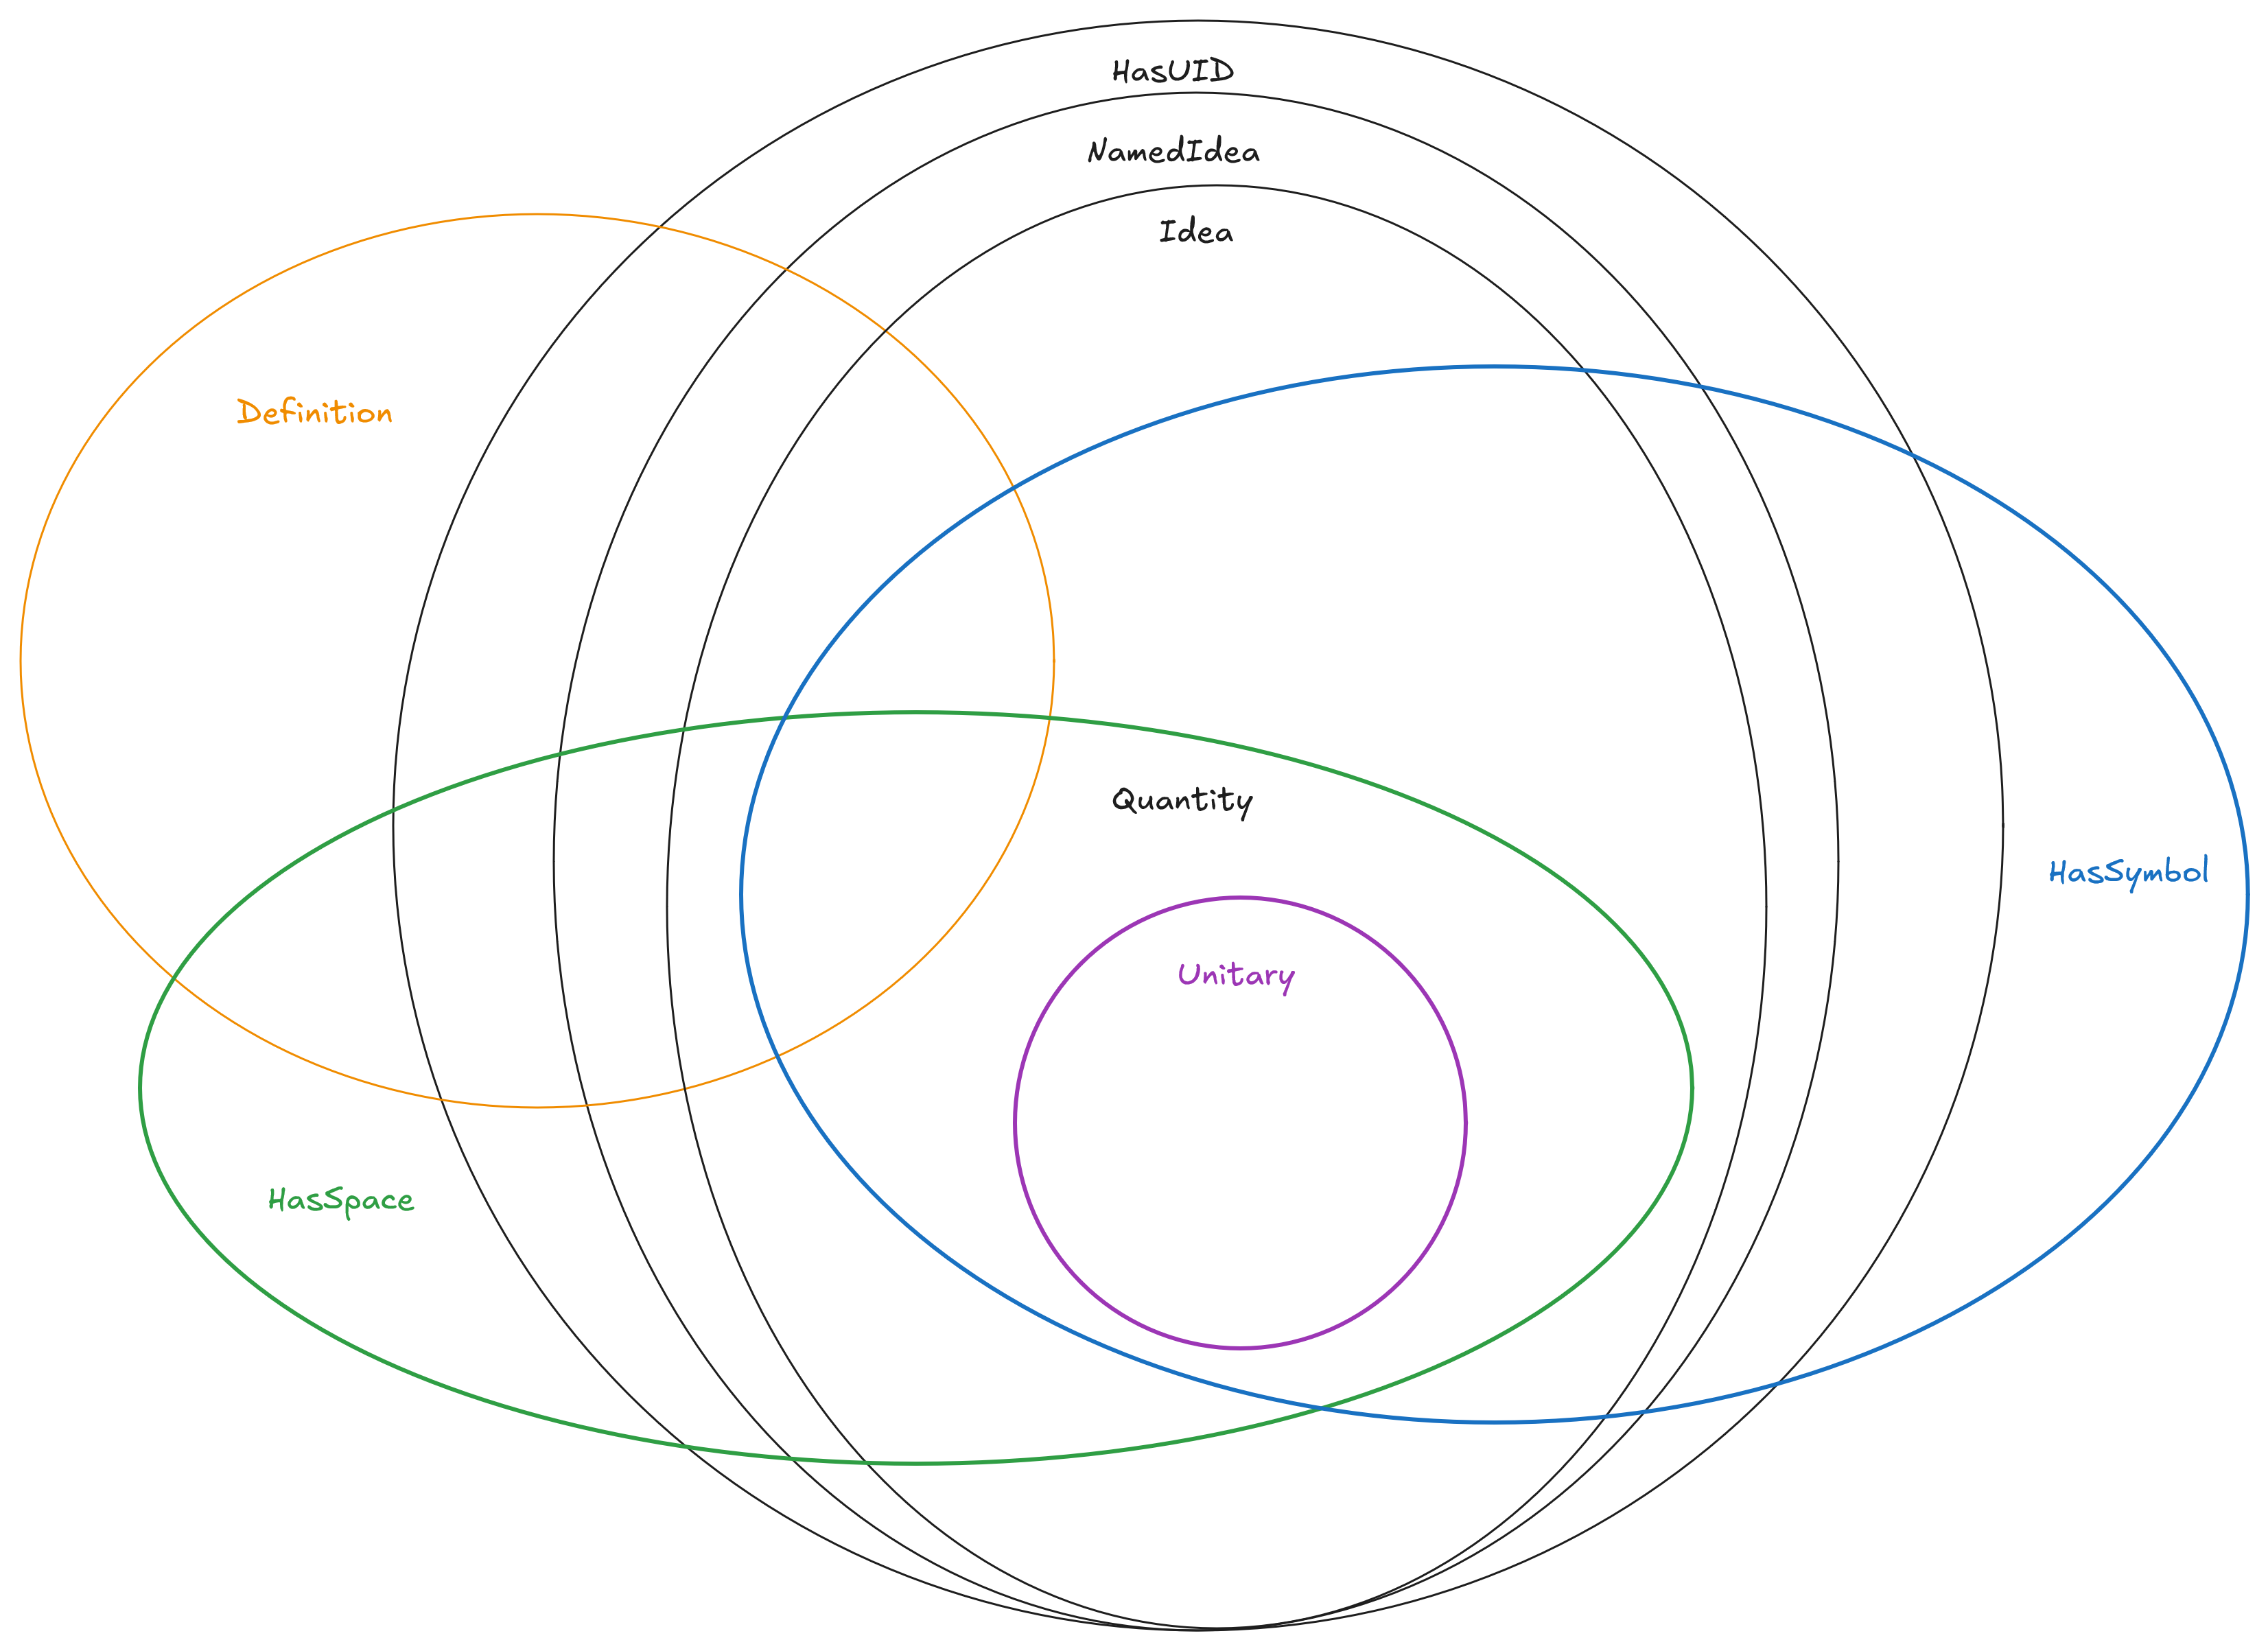
\includegraphics[width=\linewidth]{figures/ChunkClasses.png}
\end{center}}{A subset of Drasil's Chunk Classification system showing some of 
the encoded property relationships}{fig:chunkClasses}

\fig{\begin{center}
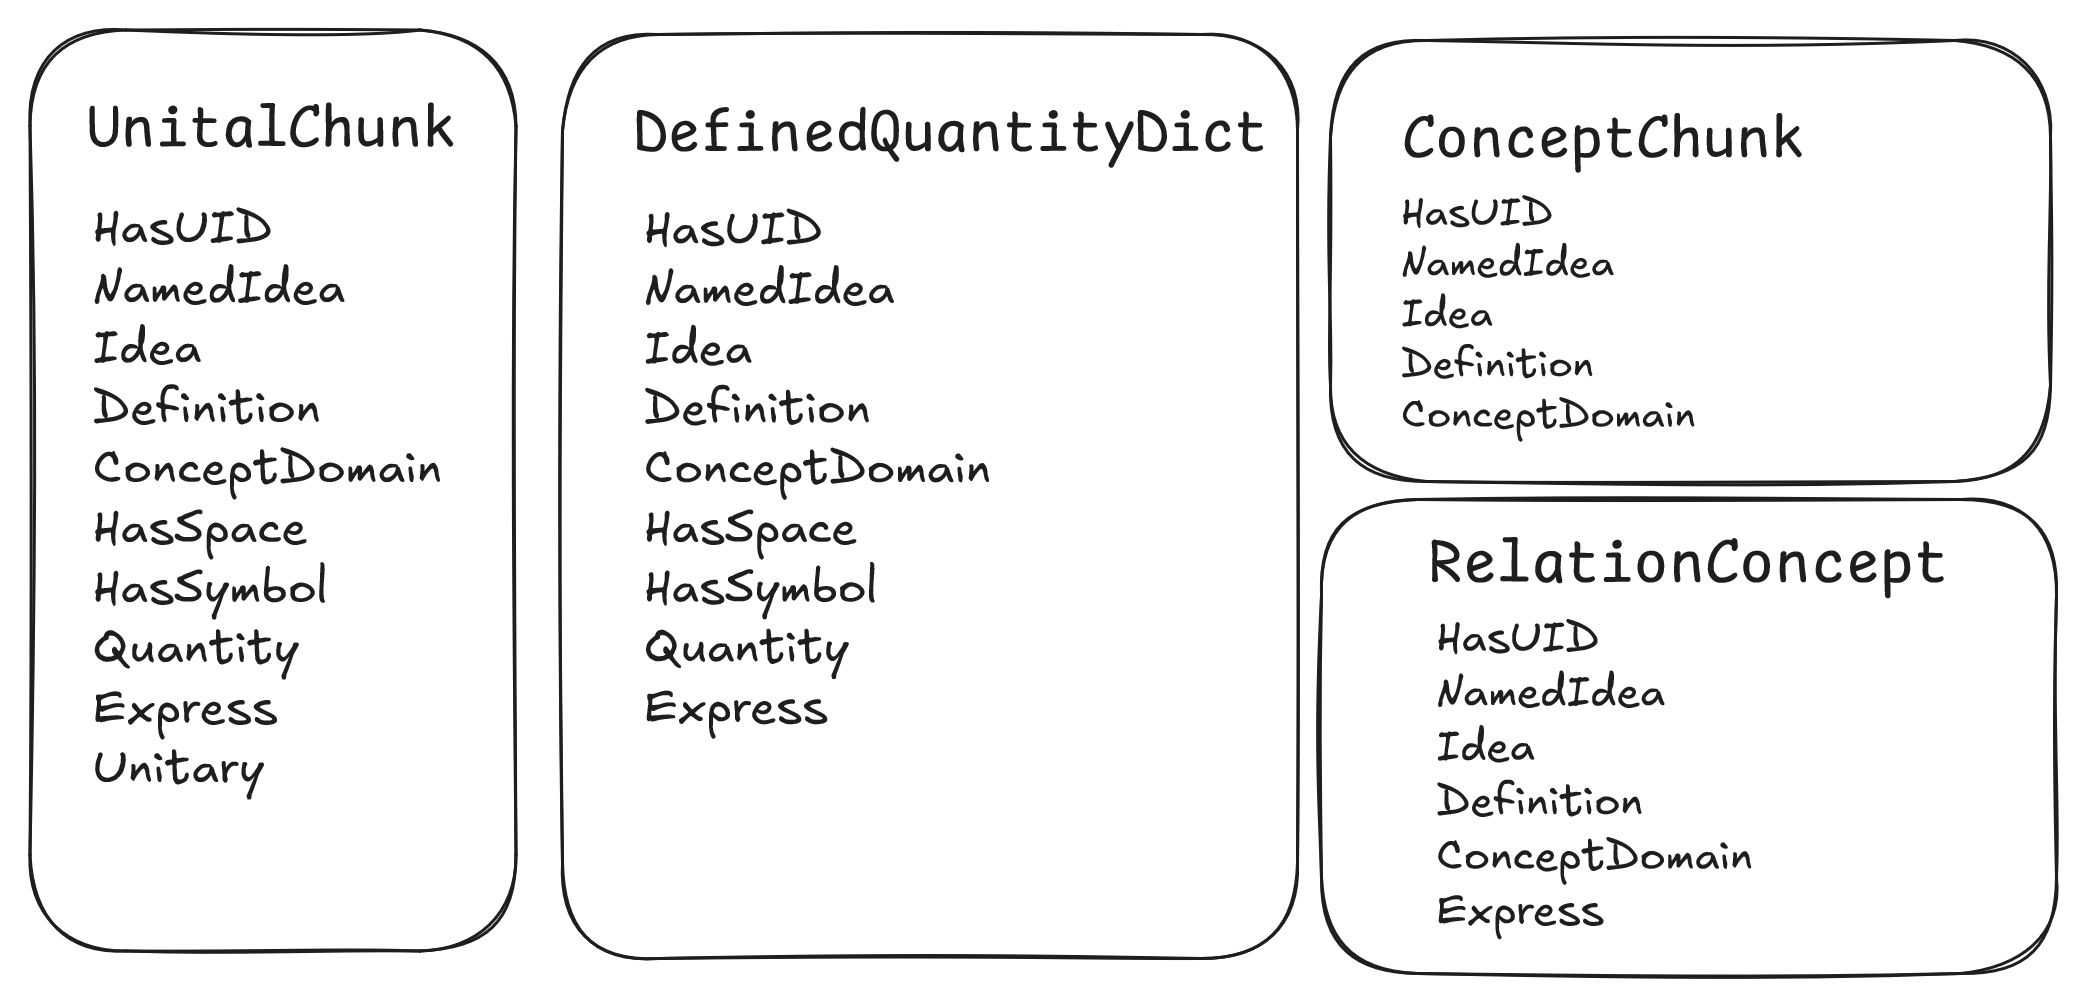
\includegraphics[width=0.75\linewidth]{figures/ChunkClassified.png}
\end{center}
}{A subset of Drasil's chunks showing how different chunks may belong to 
multiple classifications}{fig:chunksClassified}

We now have a compact, well-typed vocabulary for representing domain knowledge: 
chunks and classifications give us named concepts, quantities, units, and 
relationships that are easy to reason about. That vocabulary is only useful if 
we can turn it into artifacts people consume. To convert that vocabulary into 
artifacts people actually use, we need a way to operationalize those chunks. In 
Drasil that means using recipes.

\section{Recipes: Codifying Structure}
\label{sec:recipes}

Given our chunk classes and a compositional Expr/Sentence model in place, we 
have a knowledge core that can be selectively projected for any audience. The 
next step is thus operational: we must describe how those chunks are composed 
into artifact-specific recipes and how the recipes are rendered into concrete 
\sfs{} (documents, code, and supporting files).

Our knowledge base is essentially just a collection of chunks, which are 
themselves a collection of definitions, encoded in our Expr and Sentence DSLs. 
To generate \sfs{} we need a means to define the overall structure of the \sf{} 
as well as the knowledge projections we require to expose the appropriate 
knowledge from our chunks in a meaningful way for the target audience of that 
particular \sf{}. This is where our \emph{Recipe} DSL comes into play.

A recipe is, in it's simplest form, a specification for one or more \sfs{}. 
It is an intermediate representation of a given \sf{} and can be thought of as 
a ``little program". With it, we select which knowledge is relevant and how it 
should be organized before passing the recipe to the generator/rendering engine 
to be consumed and produce the final \sf{}. A recipe not only allows us to 
structure where knowledge should be presented, but also gives us tools for 
automatically generating non-trivial sections of our \sfs{}. For example, a 
traceability matrix can be automatically generated by traversing the tree of 
relationships between chunks within a recipe, although we'll discuss that in 
more depth in Section~\ref{sec:gen}.

As we saw in Section~\ref{sec:patterns}, there are patterns of repetition for 
the way knowledge is projected and organized within and between our \sfs{}. The 
recipe DSL has been designed to take advantage of our knowledge capture 
mechanisms to reduce unnecessary repetition and duplication. We consider the 
\sfs{} as different views of the same knowledge, and project only that which is 
relevant to the audience of the specific \sf{} our recipe applies to. For 
example, a human readable document may use symbolic mathematics notation for 
representing formulae whereas the source code would represent the same formulae 
using syntax specific to the programming language in use (or, taking an extreme 
example in the case of punch cards, punched cards). Regardless, we would define 
the underlying knowledge once in our chunks, and use the recipe DSL to select 
the representation.

\ds{A little repetitive above, but wanted to really hammer in what recipes are 
for.}

As our case studies are following templates for our \sfs{}, they give us a 
solid foundation with which to write our recipes. We already know how the 
knowledge should be organized, greatly simplifying how we can begin structuring 
our recipe DSL. The most straightforward, practical approach would be to start 
by defining a recipe for a given \sf{} type (SRS, MG, Code, etc.). Then flesh 
that out section by section, following the template as an organizational guide, 
using the patterns we discovered earlier (Section~\ref{sec:patterns}) as a 
means of avoiding unnecessary duplication. This is the approach we have chosen 
to follow, and it has lead to some interesting results.

\fig{
\codeBlock{DocDecl}{25}{42}
}{Recipe Language for SRS}{fig:recipeSRS}

As an example, let us take a look at the recipe language we have defined for an 
SRS using the \smithea{} template. Looking at the \codeH{DocSection} definition 
from Figure~\ref{fig:recipeSRS}, we can see a striking resemblance to (a subset 
of) the template's Table of Contents (Figure~\ref{fig:SRSToC}). Each section is 
defined by a datatype, which is, through a similar mechanism, decomposed into 
multiple subsections (for example, Figure~\ref{fig:recipeReqSec} shows the 
decomposition of the requirements section) which then defines the types of 
organizational structures we use for specifying the contents of a given 
subsection. When populated, the recipe specifies both the structure of our 
expected \sf{} and the knowledge (chunks) contained therein.

\fig{
\codeBlock{DocDecl}{88}{98}
}{\codeH{ReqrmntSec} Decomposition and Definitions}{fig:recipeReqSec}

As the given recipe so far has provided nothing but structure, you may be 
wondering how we populate it with the appropriate knowledge chunks to produce a 
\sf{}? For that, we should look at a specific example from one of our case 
studies (\gb{}).

\subsection{Example: SRS recipe for \gb{}}
\label{sec:glassBRSRSRecipe}

\fig{
\codeBlock{Body}{54}{55}
\vdots{}
\codeBlock{Body}{85}{126}
}{SRS Recipe for \gb{}}{fig:glassBRSRSRecipe}

The recipe for the \gb{} SRS can be seen in Figure~\ref{fig:glassBRSRSRecipe}.
This should look familiar, as it follows a similar structure to the \smithea{} 
template table of contents. We use a number of helper functions and data types 
to condense and collect the chunks we require and avoid writing any generic 
boilerplate text. The structure of the document can be rearranged to an extent, 
in that we can add, remove, or reorder sections at will by simply moving them 
around within the \codeH{SRSDecl}. We can also make choices regarding the 
display of certain types of information in the final, generated \sf{}. For 
example, we alluded to vector representations earlier 
(Section~\ref{sec:chunky}) which we currently can display using either bold
typeface or italics. This choice must be made using the \codeH{TypogConvention} 
datatype which lists the choices made (ex. 
\codeH{TypogConvention[Vector Bold]}) and is used by a relevant portion of the 
SRS recipe if vectors are included in the \sf{}. Our \gb{} example does not 
make use of this convention, however the \gp{} case study does.

As for the chunks necessary for generating the \sf{}, each section includes 
references to them through supplied lists in something we call the 
\code{C}{System Information} %System is a Haskell kw
object (Figure~\ref{fig:systemInformation}).

\fig{
\codeBlock{Body}{63}{81}
}{System Information for \gb{}}{fig:systemInformation}

The system information object uses helper functions to keep track of the lists 
of chunks necessary for filling in the sections of our \sf{}, the SRS. Each 
piece of the object consists of one or more chunks to be used in filling in the 
relevant sections. A quick description of each property can be found in 
Table~\ref{tab:siBreakdown}, but it should be noted that some of the defined 
properties are only there for convenience (and/or remain only until the next 
refinement pass) as they are derived from other chunks with the use of 
helper functions and could be inferred.

\ds{TODO: I might remove the table and just add comments to the code block 
similar to 
what's in the next section. It seems like that might be easier for readers to 
reference}

\begin{table}[]
\caption{System information object breakdown - every property is represented by 
chunks encoding given information}
\label{tab:siBreakdown}
\begin{tabular}{| P{.2\linewidth} | p{.8\linewidth}|}
\hline
 \textbf{Property} & \textbf{Chunk(s) Referenced}
\\ \hline
	\_sys & System name (ex. "\gb{}").
\\ \hline
	\_kind & \SF{} type we are defining (ex. SRS).
\\ \hline
	\_authors & List of authors of the \sf{}.
\\ \hline
	\_purpose & Purpose of the \sf{}.
\\ \hline
	\_quants & List of required quantities.
\\ \hline
	\_concepts & List of required concepts not otherwise encoded.
\\ \hline
	\_instModels & List of required instance models.
\\ \hline
	\_datadefs & List of required data definitions.
\\ \hline
	\_configFiles & List of required configuration files.
\\ \hline
	\_inputs & List of required inputs to the system.
\\ \hline
	\_outputs & List of required outputs from the system.
\\ \hline
	\_constraints & List of constraints for the system (physical and software 
	specific).
\\ \hline
	\_constants & List of required constants. 
\\ \hline
	\_sysinfodb & Database of all required chunks.
\\ \hline
	\_usedinfodb & Database of all used acronyms and symbols.
\\ \hline
	refdb & Database of all relevant external references/citations.
\\ \hline
\end{tabular}
\end{table}
 
As should be obvious, the system information object is referencing other chunks 
which have been defined elsewhere. Most definitions can be found in the 
knowledge-base, with system-specific aggregations (i.e. lists of chunks) being 
defined within the scope of the specific example project. For example, 
\codeH{iMods} referenced as the \codeH{_instModels} property is defined 
as shown in Figure~\ref{fig:iMods}, alongside the two system-specific instance 
models listed within it. The two specific instance models can be seen to be 
derived from other existing chunks, through the use of a series of helper 
functions, thus ensuring their traceability to the knowledge-base.

\fig{
\codeBlock{IMods}{18}{19}
\vdots{}
\codeBlock{IMods}{28}{33}
\vdots{}
\codeBlock{IMods}{41}{46}
}{The \codeH{iMods} definition}{fig:iMods}

Given that the system information object refers to all of the requisite chunks 
for the knowledge contained in our \sfs{} and the SRS recipe defines how that 
knowledge should be structured and organized within the \sf{}, it follows that 
those are all we should need to generate our SRS. As an aside, the complete 
recipe for the SRS specification of \gb{}\footnote{Not including chunks 
referenced from within our knowledge bases as they can be shared, reused, and 
are not necessarily specific to only this system.} including the system 
information object is contained in a single file in less than 370 lines of 
code\footnote{Including many comments, whitespace, and import statements.}. 
Teasing our results: the generated SRS in PDF format is 44 pages in length. 
This is partially due to our ability to strip away all of the common 
boilerplate text that we need not worry about right now, as that will be a 
problem for the generator (Section~\ref{sec:gen}). As it stands we have created 
the recipe language to represent what we truly want out of a recipe: a 
simplified, unnecessary-duplication-avoiding, fully traceable representation of 
our target \sf{}.

With the combination of system information and the SRS recipe we can soon move
on to creating our generator for the finished SRS document. As the other \sf{} 
recipes were developed in tandem with the SRS, they follow a similar structure 
and in the interest of brevity we will skip the breakdown of each recipe. It is 
left to the reader to investigate them by diving into our examples via the 
Drasil github. However, there is one \sf{} that is significantly different, and 
as such, we will go into more depth in discussing in the following section: the 
executable code recipe. Said recipe allows us to not only specify knowledge and 
the way we wish it structured, but also implementation choices that we would 
like to make in the final generated source code.

\subsection{Example: Executable Code recipe for \gb{}}
\label{sec:gbCodeRecipe}

As discussed in the previous section, the executable code recipe is 
fundamentally different from the documentation-heavy SRS recipe. While the SRS 
recipe focuses on organizing and projecting knowledge for human consumption, 
the executable code recipe must specify the structure and content required for 
generating working source code. This includes not only the relevant knowledge 
chunks, but also the implementation choices (modules, functions, and other 
details) necessary for code generation. 

The executable-code recipe for GlassBR somewhat mirrors the document recipe in 
structure but emphasizes implementation choices: module layout, data 
representation, target languages, optional features, and constraint-handling 
strategies. Practically, we supply the modules and computational relationships 
(the mathematical execution order), target languages (e.g. Python, C++, Java), 
modularity (single file or separated modules), data bundling (structs/classes), 
and logging/documentation options. 

The recipe for \gb{}'s executable code constructed using the 
\codeH{CodeSpec} DSL, is shown in Figure~\ref{fig:gbCodeRecipe}. 
Here, the \codeH{codeSpec} function takes three arguments:
\begin{itemize}
\item \codeH{fullSI}: the system information object, which aggregates all the 
knowledge chunks relevant to \gb{} (as described in the SRS example).
\item \codeH{choices}: a record specifying code generation options, such as 
target languages, architecture, data handling, and auxiliary files. The example 
\codeH{choices} definition for \gb{} can be seen in 
Figure~\ref{fig:gbCodeRecipe} and the object itself will be explained in more 
detail later in this section.
\item \codeH{allMods}: a list of modules to be generated, each defined in terms 
of the knowledge chunks and functions they encapsulate.
\end{itemize}

\fig{
Body.hs
\codeBlock{Body}{57}{58}
Choices.hs
\codeBlock{Choices}{13}{27}}{The Recipe for \gb's Executable 
Code}{fig:gbCodeRecipe}

\fig{
\codeBlock{CodeSpec}{41}{72}
}{The Recipe Language for Executable Code (CodeSpec)}{fig:codeSpec}

The \codeH{CodeSpec} DSL itself is defined in Figure~\ref{fig:codeSpec}, and 
a subsection of its key fields are summarized in 
Table~\ref{tab:codeSpecBreakdown}. As mentioned above, we use a helper function 
\codeH{codeSpec} to extract the appropriate fields from the system information, 
choices, and module list retaining full traceability and avoiding unnecessary 
manual duplication.

\begin{table}[]
\caption{CodeSpec object breakdown}
\label{tab:codeSpecBreakdown}
\begin{tabular} {| P{.2\linewidth} | p{.8\linewidth}|}
\hline
\textbf{Property} & \textbf{Chunk(s) Referenced} 
\\ \hline 
	pName & Program name 
\\ \hline 
	authors & List of authors 
\\ \hline 
	inputs & All input variables 
%\\ \hline 
%	extInputs & External input variables to be supplied by a file
%\\ \hline 
%	derivedInputs & Derived inputs calculated from external inputs in a single 
%	step
\\\hline 
	outputs & All output variables 
\\\hline 
	configFiles & Required configuration files 
\\\hline 
	execOrder & Mathematical definitions ordered such that they form a path 
	from inputs to outputs 
\\\hline 
	cMap & Constraints on variables 
\\\hline 
	constants & Constants used in the program 
%\\ \hline 
%	constMap & Map of the above constants used in the program for efficient 
%	lookups
\\ \hline 
	mods & List of additional code modules to generate
\\ \hline 
	sysinfodb & Database of all knowledge chunks for the given problem
\\ \hline
\end{tabular}
\end{table}

As with the SRS recipe, the code recipe references knowledge chunks defined 
elsewhere. For example, the list of input variables is defined in 
\codeH{Unitals.hs} just as they were for the SRS. Similarly, the modules to be 
generated are defined in \codeH{ModuleDefs.hs} and make reference to other 
chunks (both system specific and generic) from our knowledge-base. Looking 
into the modules, we can see the \codeH{readTableMod} module, for example, is 
defined as shown in Figure~\ref{fig:readTableMod}. This module provides a 
function for reading ASTM glass data from a file, encapsulating both the 
knowledge of the data format and the implementation logic required for code 
generation.

\fig{\codeBlock{ModuleDefs}{30}{39}}
{The \codeH{readTableMod} module definition}{fig:readTableMod}

While the encapsulation of knowledge in chunks is interesting, we have seen it 
before in the SRS recipe example. What is novel to the code recipe is the 
\codeH{Choices} object. As mentioned above, it contains the outcome of very 
important implementation-level choices that must be made to generate the 
executable code. The definition for the \codeH{Choices} object can be seen in 
Figure~\ref{fig:choicesDefn} and a breakdown of each property can be found in 
Table~\ref{tab:choicesBreakdown}.

\fig{\codeBlock{ChoicesDefn}{26}{42}}{The \codeH{Choices} object 
definition}{fig:choicesDefn}

\begin{table}[]
\caption{Choices object breakdown}
\label{tab:choicesBreakdown}
\begin{tabular} {| P{.2\linewidth} | p{.8\linewidth}|}
\hline
\textbf{Property} & \textbf{} 
\\ \hline 
	lang & List of target languages
\\ \hline 
	architecture & Architecture of the generated code. Includes modularity 
	(whether to split into modules or generate a single flat file) and 
	implementation type (library to be consumed or standalone program)
\\ \hline 
	dataInfo & Data structure and representation choices. (Ex. bundle inputs 
	together into a class/struct, define constants inline, use the languages 
	constant mechanism, etc.)
\\\hline 
	maps & Mapping of Drasil concepts and mathematical spaces to code concepts 
	and types in the target language(s) (ex. One could map the concept of $\pi$ 
	with the language's built-in $\pi$ and the $\mathbb{R}$ space to 
	single/double precision floating point numbers)
\\\hline 
	optFeats & Choices for optional features including documentation (comments 
	and verbosity), logging, and auxiliary files.
\\\hline 
	srsConstraints & Constraint violation behaviour. Can be used to specify 
	whether to throw a warning or exception for physical/software constraints 
	independently.
\\\hline 
	extLibs & List of external libraries to use (ex. for solving specific 
	classes of mathematics problems). These libraries are external to Drasil 
	and give the option for users to link to optimized, well-established 
	libraries rather than reimplementing them from scratch in Drasil.
\\\hline 
\end{tabular}
\end{table}

With our understanding of the \codeH{Choices} object, we can now look back at 
the \gb{} example (Figure~\ref{fig:gbCodeRecipe}) and understand what 
specific implementation choices have been made. First off, the \codeH{lang} 
property has been set so the generated code will be output in five different 
programming languages: Python, C++, C\#, Java, and Swift. This is a good 
demonstration of Drasil's ability to target multiple platforms from a 
single knowledge base. The \codeH{architecture} is configured as modular, with 
input-related functions separated into their own modules (
\codeH{Modular Separated}), and the implementation type is set to 
\codeH{Program}, meaning the generated code will be a complete, runnable 
application rather than just a library. 

For data representation, the \codeH{dataInfo} field specifies that inputs 
should be bundled together (for example, as a class or struct), constants 
should be defined inline within the code, and the language's constant mechanism 
should be used where possible. The \codeH{optFeats} field enables comprehensive 
documentation by including function, class, and module-level comments, but sets 
the documentation verbosity to quiet and hides date fields in the generated 
comments. Logging is also enabled for both variable assignments and function 
calls, with all logs directed to a file named \codeH{log.txt}. Additionally, 
the auxiliary files generated include a sample input file (pointing to a real 
data file) and a \codeH{README}, supporting both usability and reproducibility. 

Finally, the \codeH{srsConstraints} field is set so that any violation of 
software or physical constraints will result in an exception, ensuring that 
errors are caught and handled strictly during execution. This configuration 
ensures that the generated \gb{} code is well-documented, maintainable, and 
ready for use in a variety of environments.

By structuring the executable code recipe in this way, Drasil ensures that all 
generated code is fully traceable to the underlying knowledge base and any 
external libraries. Any change in the knowledge chunks or their relationships 
is automatically reflected in the generated code, just as it is in the 
documentation. This approach minimizes duplication, maximizes consistency, and 
enables reliable code generation for scientific computing applications.

\subsection{Operational Summary}

Having established how Drasil captures, organizes, and operationalizes 
knowledge through both documentation and executable code recipes, we are now 
poised to explore the final step in Drasil's operation: turning these 
structured specifications into tangible \sfs{}. The next piece of the story 
will show how Drasil takes these recipes and, through a unified process, 
produces the diverse \sfs{} required by different stakeholders. In the 
following section, we delve into the mechanisms and philosophy behind Drasil's 
generation and rendering, showing how the framework brings together all the 
ingredients we've discussed to deliver consistent, traceable, and maintainable 
\sfs{}.

\section{Cooking it all up: Generation/Rendering}
\label{sec:gen}

The previous sections have detailed how Drasil captures domain knowledge as 
chunks, organizes it via a robust hierarchy, and structures it into recipes 
that specify the desired artifacts. In this section, we focus on the final 
stages of the generation pipeline: \emph{rendering} and \emph{assembly}. These 
stages are responsible for transforming the intermediate representations 
(recipes and their referenced chunks) into tangible, concrete, consumable 
\sfs{}, such as documents and executable code.

\subsection{Rendering: From Abstract Structure to Concrete Formats}

At its core, Drasil treats recipes as ``little programs". Rendering in Drasil 
refers to the process by which these abstract, language-agnostic structures 
defined in recipes are transformed into specific output formats suitable for 
end-users and stakeholders. This stage bridges the gap between the high-level, 
reusable knowledge representations and the diverse forms required for practical 
use (ex. \LaTeX{}, HTML, PDF, or source code in various programming 
languages).Drasil achieves this through a set of dedicated \emph{printers} and, 
for code, through the use of the General Object-Oriented Language 
(GOOL)\cite{??} library. Each printer is designed to interpret the structured 
data produced by the recipe and knowledge projection stages and emit output in 
the desired format, handling both content and layout\footnote{To some respect, 
depending on the desired output format. For instance, \LaTeX handles the 
majority of the finished \sf{}'s layout where Drasil generates the content}.

\subsubsection{Document Rendering: Printers and Output Engines}
For documentation artifacts (such as SRS or Module Guide), Drasil provides 
specialized printers for each supported format:
\begin{itemize}
    \item \codeH{genTeX} in \codeH{Language.Drasil.TeX.Print} --- renders the 
    document as \LaTeX{} source, suitable for PDF generation.
    \item \codeH{genHTML} in \codeH{Language.Drasil.HTML.Print} --- produces 
    HTML for web-based consumption.
    \item \codeH{genJSON} in \codeH{Language.Drasil.JSON.Print} --- outputs a 
    machine-readable JSON representation, supporting further processing or 
    integration.
\end{itemize}

Each printer traverses the recipe structure, visiting each section and 
sub-section, and calls formatting routines appropriate to the target format. 
For example, a Data Definition chunk will be rendered as a LaTeX table row, an 
HTML table entry, or a JSON object, depending on the printer invoked.
\subsubsection{Example: SRS to \LaTeX{}}
As a concrete illustration, consider the printing of the \gb{} SRS to 
\LaTeX{}. The process begins with the invocation of the \codeH{genTeX} 
function, which recursively walks the document tree produced by the recipe, 
emitting \LaTeX{} code for sections, equations, and tables. 
Figure~\ref{fig:genTeX} shows the entry point to this process.

\fig{\codeBlock{TeXPrint}{41}{44}}{\codeH{genTeX} function for LaTeX 
rendering}{fig:genTeX}

\subsubsection{Code Rendering: GOOL and Target Language Emission}
For executable code artifacts, Drasil uses GOOL\cite{??} as an intermediate 
layer. GOOL provides a collection of type-safe combinators and abstractions for 
representing object-oriented and procedural constructs in a language-agnostic 
manner. The code recipe (ex. a \codeH{CodeSpec}) is first translated into a 
GOOL abstract syntax tree (AST), which is then emitted as source code in one or 
more target languages. For brevity we will not get into the implementation 
details regarding Drasil's use of GOOL, as those have been covered in other 
works \cite{??} \ds{Someone else's thesis covered this yeah? I don't want to 
make it sound like I wrote this part, but still want to give an overview}.

In brief, the code emission process follows a straightforward translation 
process: The code recipe and its referenced chunks are traversed to construct a 
GOOL AST, representing classes, functions, variables, and control flow; The 
GOOL backend is invoked for each specified target language, translating the AST 
into concrete source code (ex. Python, C++, Java, C\#); Auxiliary files (such 
as README, Doxygen config, and sample input files) are generated via dedicated 
routines.

\subsubsection{Example: Emitting \gb{} Code in Python}
For \gb{}, suppose the code recipe specifies Python as a target. The 
generation process calls \codeH{generateCode} in 
\codeH{Language.Drasil.Code.Imperative.Generator}, which constructs the GOOL 
AST and then emits Python code by invoking the Python backend. The resulting 
code includes all functions, data structures, and comments specified in the 
recipe and choices object, as well as any automatically generated traceability 
links (ex. comments referencing requirements or data definitions). 
Figure~\ref{fig:generateCode} shows the relevant code path.

\fig{\codeBlock{ImperativeGenerator}{98}{113}}{generateCode and genPackage for 
code rendering}{fig:generateCode}

\subsection{Assembly: Producing the Final \SF{} Set}
Once rendering is complete, the generated document or code sections must be 
assembled into coherent artifacts ready for distribution and use. Assembly 
includes writing the primary artifacts to disk (ex. *.tex, *.html, *.py, *.cpp 
files), generating auxiliary files (ex. Makefiles, CSS, README, example input 
files), linking cross-references, and ensuring the integrity of tables, 
figures, and code modules. The remainder of this section illustrates these 
steps in practice.

\subsubsection{Example: SRS Assembly}

After rendering the \gb{} SRS to \LaTeX{} via the \codeH{genTeX} function seen 
in Figure~\ref{fig:genTeX}, the~\codeH{prntDoc'}~function, 
Figure~\ref{fig:prntDocPrime}, writes the source file, while \codeH{prntMake}, 
Figure~\ref{fig:prntMake}, generates a Makefile for automated PDF compilation. 
The resulting directory contains a fully cross-referenced, typeset-ready SRS 
and all supporting files.

\fig{\codeBlock{Generate}{56}{60}}{\codeH{prntDoc'} function for document 
output}{fig:prntDocPrime}

\fig{\codeBlock{Generate}{68}{73}}{\codeH{prntMake} function for document 
output}{fig:prntMake}

\subsubsection{Example: Code Assembly}

Once the code has been rendered through the GOOL pipeline into target-language 
text, the next stage is to assemble the resulting files into a coherent project 
structure. In this case, \codeH{createCodeFiles} 
(Figure~\ref{fig:createCodeFiles}) is called to write each generated source 
file and all auxiliary documentation to disk using consistent directory and 
naming conventions. For multi-language builds, this process is repeated for 
each target language, ensuring consistency across all output.

In essence, this stage performs for code what the SRS assembly stage does for 
documentation: it gathers the individually generated fragments and organizes 
them into a complete, ready-to-use product. The result comprises all files 
necessary for the generated system source code, build instructions, and 
supporting assets. They are generated and ready for compilation or integration 
into a development environment. Because these outputs are directly derived from 
the same knowledge base that informed the SRS, Drasil ensures that the 
implementation remains consistent with the documentation.

\fig{\codeBlock{CodeGeneration}{28}{38}}{createCodeFiles for code 
output}{fig:createCodeFiles}

\subsection{A \gb{} Example: From Chunk Definition to Final SRS Rendering}

To illustrate the rendering and assembly process, we follow a single chunk 
through each step of generation in the \gb{} SRS. Earlier, we 
described how the SRS recipe for \gb{} is constructed by specifying the 
document structure and referencing the necessary knowledge chunks through the 
system information object (see Section~\ref{sec:glassBRSRSRecipe}). Now we 
observe the journey of the dimensionless load chunk ($\hat{q}$), from 
its definition in the knowledge base to its appearance as typeset-ready \LaTeX 
formatted text in the generated SRS.

\subsubsection{Step 1: Knowledge Capture}

The definition of $\hat{q}$ is captured in the Drasil knowledge base as a 
chunk (Figure~\ref{fig:qhatChunkDef}). This chunk contains all necessary 
information: a unique identifier, symbol, natural language description, units, 
and the defining mathematical expression.

\fig{
\codeBlock{DataDefs}{130}{142}}{Definition of $\hat{q}$ as a chunk in the 
\gb{} knowledge base}{fig:qhatChunkDef}

\subsubsection{Step 2: Recipe Specification}

In this step, the previously defined $\hat{q}$ chunk is referenced and included 
in the system information and recipe for the \gb{} SRS. Here, $\hat{q}$ is 
added to the list of Data Definitions (can be seen as \codeH{GB.dataDefs} 
in Figure~\ref{fig:systemInformation}), which will later be used to populate 
the relevant sections (Table of Symbols, Data Definitions, Traceability Matrix, 
etc.) of the document. This step is about specifying what 
knowledge is relevant and where it should appear, not about how it is rendered.

\subsubsection{Step 3: Generation and Rendering}
When the generator is invoked to produce the SRS (ex. as a \LaTeX{} document), 
it traverses the recipe, visiting each section. For the Data Definitions 
section, it projects the full definition of $\hat{q}$, including its symbol, 
description, units, and defining equation. For the Table of Symbols, it 
projects only the symbol, a brief description, and the units. The rendering 
engine formats these projections according to the conventions of the target 
output.

\fig{\TeXBlock{GlassBR_SRS}{750}{799}}{Raw generated \LaTeX of the $\hat{q}$ 
Data Definition}{fig:rawDD}

During rendering, the SRS generator traverses the recipe and, for each chunk 
referenced, projects and formats it for the target output. 
For the Data Definitions section, it projects the full definition of $\hat{q}$, 
including its symbol, description, units, and defining equation 
(Figure~\ref{fig:rawDD}). For the Table of Symbols, it projects only the 
symbol, a brief description, and the units. The rendering engine formats these 
projections according to the conventions of the target output (as a \LaTeX 
table or section).

\subsubsection{Step 4: Assembly and Output}

Finally, the rendered sections are assembled into the complete SRS artifact. 
Cross-references are automatically generated, so that, for example, references 
to $\hat{q}$ in Instance Models or Requirements link back to its definition in 
the Data Definitions and/or Table of Symbols. Auxiliary materials, such as the 
Table of Units and Table of Abbreviations, if required, are generated by 
traversing the relevant lists in the system information object, ensuring 
consistency and completeness. The completed document is output as a 
\texttt{.tex} file with $\hat{q}$ fully integrated and accessible 
alongside all other relevant auxiliary files (ex. \texttt{.bib} file for 
citations). A makefile is also generated to 
enable the user to easily create a human-readable PDF file from the \LaTeX 
source and auxiliary files.

\subsection{Multiple Renderings from a Single Source: From Chunk to Code}

As a continuation of the previous section’s example, we now follow the 
dimensionless load $\hat{q}$ from its knowledge base definition through to its 
realization in the generated source code. This example concretely demonstrates 
how Drasil’s single-source-of-truth approach ensures that mathematical concepts 
are faithfully and consistently reflected in both documentation and code 
artifacts.

\subsubsection{Referencing $\hat{q}$ in the Code Recipe}

Recall that $\hat{q}$ was previously defined as a chunk containing its symbol, 
natural language description, units, and mathematical formula (see 
Figure~\ref{fig:qhatChunkDef}). In the process of generating executable code, 
this chunk is referenced in the system information object (\codeH{fullSI}) and 
included in the \codeH{CodeSpec} recipe for 
\gb{}(Figure~\ref{fig:gbCodeRecipe}). The recipe dictates which variables and 
formulas are required in the target program, and provides implementation-level 
choices such as type mapping and function structure.


\subsubsection{Rendering via GOOL}

During code generation, Drasil translates the recipe and referenced chunks into 
a GOOL (General Object-Oriented Language) intermediate representation. The 
$\hat{q}$ chunk, for example, is mapped to a function definition within the 
GOOL AST, preserving its formula and metadata. This intermediate form enables 
Drasil to emit code in multiple target languages without duplicating logic. As 
GOOL is not the subject of this thesis, we will elide the GOOL-specific details 
and continue down the code generation pipeline.

\subsubsection{Generated Source Code}

In the final step, the GOOL backend emits concrete code for $\hat{q}$ in each 
selected language. For example, in Python, $\hat{q}$ appears as a function 
computing its value from its dependencies(Figure~\ref{fig:qhatPython}) just as 
we've seen before in Figure~\ref{fig:gbrsrccalc}. The generated code maintains 
traceability through naming conventions and comments drawn from the original 
chunk. The final python output can be seen in Figure~\ref{fig:qhatPython}.

\fig{\pyBlock{GenCalculations}{34}{40}}{$\hat{q}$ as defined in the generated 
python code}{fig:qhatPython}

\subsubsection{Discussion}

This example demonstrates how Drasil’s architecture ensures that any update to 
the definition or formula of $\hat{q}$ is automatically propagated to the 
generated code, just as it is to documentation artifacts. The use of a 
knowledge-centric pipeline, combined with language-agnostic intermediate 
representations, guarantees consistency and traceability throughout the 
software system. Changes need only be made once, and are reflected everywhere 
$\hat{q}$ appears, reducing maintenance cost and risk of error.

\subsection{Summary}
In summary, rendering and assembly are the final, crucial steps that 
operationalize Drasil's knowledge-centric approach and translate the abstract 
representations produced by our chunks and recipes into practical, high-quality 
\sfs{}. The examples from \gb{} demonstrate the practical effectiveness of this 
approach for both documentation and code.

The next section will discuss how iteration and refinement were used in the 
creation of Drasil, and how the framework enables rapid evolution of both 
knowledge and artifacts.

\section{Iteration and refinement}
\label{sec:iterefine}

With the understanding of Drasil's structure and implementation, we can now 
discuss continuous improvement. The development of Drasil did not follow 
anything even remotely close to the waterfall model of software development. If 
anything its development began with a simple set of ideas that created a basis 
for refinement. That is to say: it \emph{barely} worked.

We approached the development knowing the scope was far too large to plan out 
all the details ahead of time (in any reasonable time-frame), and made 
conscious choices on compromises we were willing to accept to get a minimum 
viable framework and continuously improve upon it, similar to agile software 
development practices. As such, and as we have eluded to throughout this and 
the previous chapter, we took a very practical approach to development by 
starting with a known-good state (our case studies), generalizing as much as 
possible (as seen in Chapter~\ref{c:process}) to distill what we needed to 
understand to generate software, and updating the framework as our assumptions 
were challenged or found wanting. Finding holes is a lot easier when you 
constantly step in them.

Many of our updates involved modifying implementation details (such as Chunk 
types, combinators, and adding entirely new concepts) when we started looking 
at the various case study domains and determining how we'd distill and capture 
the knowledge necessary to reproduce those case studies.

Throughout this process of iterative refinement, we inevitably found a number 
of places to improve upon the existing case studies and applied those changes 
to our known-good state. We found errors and undocumented assumptions in the 
case studies that caused us to rework and improve them for the future. 
Crucially, moving the case studies into Drasil made those mistakes trivial to 
locate and correct. A representative example is the SSP symbol inconsistency 
(Issue \#348 on the GitHub issue tracker). The original SSP SRS used the pair 
$S_i$ and $P_i$ (mobilized shear stress and resistive shear force respectively) 
in one place and later switched $S_i$ to $\tau_i$ (resistive shear stress). 
$\tau_i$ was also omitted from the Table of Symbols. To reiterate, that 
inconsistency existed in the original case study and was not a generator bug 
but an error in the source document we had accepted as our starting point. Once 
the SSP material was encoded as chunks in Drasil the fix was minimal: ensure we 
had encoded the correct definitions of $S_i$, $P_i$, and $\tau_i$ and used them 
in the appropriate equations. Then the correction automatically propagated to 
all generated artifacts (Table of Symbols, cross‑references, and any code that 
referenced the symbol).

We also noticed a unit mismatch during the investigation of that issue, which 
sparked some confusion until we determined there was an unspecified assumption 
of 1m depth ``into the page" for one of the equations. That assumption was 
later captured and encoded into the specific knowledge for that family of 
software systems as well. Overall the effort to fix both of these related 
issues was essentially a focused edit to a minuscule subset of the captured 
knowledge, not a widespread rewrite.

This pattern repeats across many issues: we would find a mismatch between a
case study and our Drasil output, or some as-yet unencoded knowledge (ex. 
implicit assumptions) that made the generated artifacts inconsistent or 
unclear, update the chunk(s) that encoded the offending knowledge, and 
re‑generate. That workflow was the dominant mode of refinement of the original 
case studies and their Drasil implementations. It kept fixes small, localized, 
and low cost while producing broad, immediate benefits in every artifact that 
depended on the corrected knowledge.

As Drasil encodes both semantics (definitions, units, relations) and 
presentation choices (how a chunk is projected), correcting semantics upstream 
was also used to eliminate downstream inconsistencies with, often, minimal 
engineering effort. One example of this is changing our Chunk hierarchy to 
include derived-unit chunks. After we determined the need for \codeH{Unital} 
chunks which tied units to captured knowledge, it was obvious that the units 
themselves would need to be able to represent their relationships, particularly 
for those derived from standard SI units (ex. $m/s^2$). This involved the 
addition of new combinators for creating \codeH{UnitDefn} chunks (examples of 
some of these combinators have already been shown in Figure~\ref{fig:accelU}).

In short, we learned how to improve Drasil by trying to reproduce existing case 
studies, encoding what we needed as chunks, and then correcting or extending 
the chunks when mismatches were discovered. Fixes were either small edits to 
the knowledge base (cheap to apply, and automatically, consistently propagated 
to all generated outputs) or an extension of the way we chose to capture 
knowledge (new chunk types or combinators to encode previously un-encodable 
knowledge or relationships between chunks).

\section{Summary}

In this chapter we have described the architecture and implementation choices 
that make Drasil practical: a knowledge‑centric pipeline built from reusable, 
typed ``chunks'', lightweight DSLs for expressions and natural language 
fragments, and a recipe language that codifies how knowledge is projected into 
concrete artifacts. The design is intentionally pragmatic: we capture what is 
needed to reproduce real case studies, provide well‑typed building blocks for 
assembling that knowledge, and offer generators (printers and the GOOL back 
end) that render the same source into multiple, consistent outputs. The result 
is a single source of truth that spans documentation and executable code.

By separating the concerns of knowledge capture, structuring, rendering, and 
assembly, Drasil ensures that \sfs{} remain maintainable, consistent, 
traceable, and free of unnecessary manual duplication from their high-level 
specification down to their concrete instances. All of which increases 
confidence in the resulting software systems.

The chunk hierarchy and its classification system give us the levers we need to 
balance expressivity and reuse. Simple chunks (NamedChunk, ConceptChunk) let us 
represent terminology and definitions; richer chunks (UnitalChunk, UnitDefn, 
DataDefn, InstanceModel) let us attach units, symbols, and executable 
expressions; and the Expr / Sentence DSLs give us language‑agnostic ways to 
express mathematics and narrative. Recipes then select and arrange those chunks 
for particular stakeholders so that the same underlying knowledge can be 
rendered as an SRS, a module guide, or multi‑language source code with full 
traceability between pieces.

The iterative approach to Drasil's development ensured modularized components 
that improve extensibility and maintainability of the system as a whole, as 
well as continuous refinement and expansion of the system's capabilities. A key 
practical lesson is that encoding case studies into Drasil exposes errors 
and implicit assumptions in the original artifacts but makes them trivial to 
fix. Fixes are usually local edits to the knowledge base and those edits 
automatically propagate through all generated artifacts. This demonstrates the 
principal payoff of the single‑source, chunk‑based approach: small, cheap 
changes at the source yield broad, consistent improvements everywhere.

Drasil is not a universal solution — it is a tool targeted at domains where the 
models are well understood, long‑lived, and shared across multiple 
stakeholders. Within that scope, Drasil shifts effort from repetitive editing 
of many artifacts to careful modeling of domain knowledge. The framework we 
have presented allows that modeling to pay dividends immediately (consistent 
documents and code) and continuously (streamlined evolution through iteration 
and refinement).